\tikzset{
    ->, 
    level distance = 22em,
    minimum size=2em,
    %edge from parent/.style={draw,thick},
    level 1/.style={sibling distance=6em},
    level 2/.style={sibling distance=3em},
    thick/.style = {line width=1.5pt},
    extra thick/.style = {line width=3.5pt},
    red node/.style={shape=circle,draw=red,fill=red!40,thick,inner sep=1.2},
    blue node/.style={shape=circle,draw=blue,fill=blue!40,thick,inner sep=1.2},
    line/.style={-stealth, thick, draw}
  } 

\tikzstyle{round}=[thick,draw=black,circle]

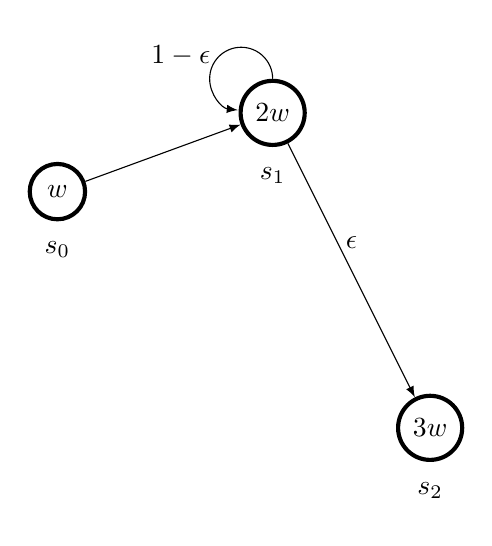
\begin{tikzpicture}[auto,node distance=58mm,>=latex]
    \tikzstyle{round}=[thick,draw=black,circle]
    \node[round, label=below:$s_0$] (s0) {$w$};
    \node[round, label=below:$s_1$, above=10mm, right=23mm] (s1) {$2w$};
    \node[round, label=below:$s_2$, below=30mm, right=43mm] (s2) {$3w$};

    \draw (s0) -> (s1);
    \draw [->] (s1.90) arc (0:264:4mm) node[midway,left]{$1-\epsilon$}; 
    \draw (s1) -> (s2) node[midway,above]{$\epsilon$};

%    \path [line] (s1.90) -- node [text width=1.5cm,midway,above,align=center] {$1-\epsilon$} (s1); %arc (0:264:4mm);

%    \path [line] (s1) -- node [text width=2.5cm,midway,above,align=center ] {$\epsilon$} (s2);

\end{tikzpicture}
